\documentclass[12pt]{article}

\usepackage{sbc-template}
\usepackage[utf8]{inputenc}
\usepackage{amsmath}
\usepackage{graphicx}
\usepackage{booktabs}
\usepackage{tabularx}
\usepackage{array}
\usepackage{xcolor}
\usepackage{listings}
\usepackage{float}
\usepackage{enumitem}
\usepackage{tikz}
\usetikzlibrary{positioning,arrows.meta,shapes.multipart,fit}
\usepackage{url}
\usepackage[hidelinks]{hyperref}

% Português: usa o babel quando o idioma estiver instalado (Overleaf, MiKTeX, TeX Live completo)
\IfFileExists{brazil.ldf}{%
  \usepackage[brazil]{babel}%
}{%
  \usepackage[english]{babel}%
  \addto\captionsenglish{%
    \renewcommand{\figurename}{Figura}%
    \renewcommand{\tablename}{Tabela}%
    \renewcommand{\refname}{Referências}%
    \renewcommand{\lstlistingname}{Código}}%
  \hyphenpenalty=10000 \exhyphenpenalty=10000 \sloppy
}

\graphicspath{{figuras/}}
\setlist{itemsep=2pt,topsep=4pt,parsep=0pt}
\renewcommand{\arraystretch}{1.15}

% Listagens de código
\definecolor{fundocodigo}{HTML}{F4F5F7}
\definecolor{palavra}{HTML}{1B2A4A}
\definecolor{comentario}{HTML}{6B7079}
\definecolor{texto}{HTML}{9A3B2E}
\lstset{
  basicstyle=\ttfamily\scriptsize,
  backgroundcolor=\color{fundocodigo},
  keywordstyle=\color{palavra}\bfseries,
  commentstyle=\color{comentario}\itshape,
  stringstyle=\color{texto},
  frame=single, rulecolor=\color{fundocodigo},
  framesep=4pt, xleftmargin=4pt, xrightmargin=4pt,
  breaklines=true, showstringspaces=false, columns=fullflexible,
  aboveskip=8pt, belowskip=4pt,
  literate={á}{{\'a}}1 {é}{{\'e}}1 {í}{{\'i}}1 {ó}{{\'o}}1 {ú}{{\'u}}1
           {ã}{{\~a}}1 {õ}{{\~o}}1 {ç}{{\c{c}}}1 {ê}{{\^e}}1 {â}{{\^a}}1 {ô}{{\^o}}1
           {Á}{{\'A}}1 {É}{{\'E}}1 {Í}{{\'I}}1 {Ç}{{\c{C}}}1 {Ã}{{\~A}}1
}
\lstdefinelanguage{CSharp}{
  morekeywords={var,from,in,join,on,equals,into,select,new,where,if,return,await,async,public,null,true,false,string,int,bool,DateTime,decimal,Task,IActionResult,orderby},
  sensitive=true, morecomment=[l]{//}, morestring=[b]"
}
\lstdefinelanguage{JS}{
  morekeywords={async,await,function,let,const,return,if,for,of,new,throw,true,false,null},
  sensitive=true, morecomment=[l]{//}, morestring=[b]", morestring=[b]', morestring=[b]`
}
\lstdefinelanguage{SQLsimples}{
  morekeywords={SELECT,FROM,INNER,LEFT,JOIN,ON,AS,WHERE,IS,NULL,ISNULL},
  sensitive=false
}

\title{RentalSystem: front-end web integrado à API\\de uma locadora de veículos}

\author{Kaike Yoshioka}

% TODO: confira o nome da instituição e da disciplina antes de entregar
\address{Análise e Desenvolvimento de Software -- Tecnologias para Análise e Desenvolvimento\\
  {}[Nome da instituição]}

\email{kaike.yoshioka1703@gmail.com}

\begin{document}

\maketitle

\begin{abstract}
This paper presents the web front-end of RentalSystem, a car rental system whose database and
RESTful API (ASP.NET Core, Entity Framework Core and SQL Server Express) were built in the first
practical assignment. Based on mid-fidelity wireframes designed in Figma, the front-end was
implemented with HTML, CSS, Bootstrap and plain JavaScript, consuming the API exclusively through
the Fetch API. It provides create, read, update, delete and search screens with custom filters on
at least two fields for each of the five entities, a rental return workflow that computes the total
amount, and a reports screen that uses the five join-based routes of the back-end.
\end{abstract}

\begin{resumo}
Este artigo apresenta o front-end web do RentalSystem, um sistema de locadora de veículos cujo
banco de dados e API RESTful (ASP.NET Core, Entity Framework Core e SQL Server Express) foram
construídos no primeiro trabalho prático. A partir de wireframes de média fidelidade feitos no
Figma, o front-end foi implementado com HTML, CSS, Bootstrap e JavaScript, consumindo a API apenas
pela Fetch API. Ele oferece telas de cadastro, edição, exclusão e pesquisa com filtros
personalizados em pelo menos dois campos para cada uma das cinco entidades, um fluxo de devolução
que calcula o valor total do aluguel e uma tela de consultas que usa as cinco rotas com JOIN do
back-end.
\end{resumo}

\section{Introdução}

Uma locadora de veículos precisa controlar a frota, os clientes, as locações e os pagamentos.
No Trabalho Prático~1 foi desenvolvido o \emph{back-end} desse sistema, chamado RentalSystem:
a modelagem do banco de dados, a implementação das entidades com Entity Framework Core, uma API
RESTful em ASP.NET Core com operações de CRUD para todas as entidades, cinco rotas de consulta que
usam junções entre tabelas e a documentação dos testes no Swagger.

Até então, porém, o sistema só podia ser usado por quem soubesse montar requisições HTTP. O
objetivo deste segundo trabalho é construir o \emph{front-end} que torna o RentalSystem utilizável
por um atendente da locadora: telas para cadastrar, editar, excluir e pesquisar cada entidade,
filtros personalizados e a visualização das consultas do banco, sempre integrando as telas à API
já existente, sem dados estáticos.

O restante do texto está organizado assim: a Seção~\ref{sec:modelagem} retoma o problema e a
modelagem; a Seção~\ref{sec:arquitetura} descreve a arquitetura e as tecnologias; a
Seção~\ref{sec:wireframes} apresenta os wireframes; a Seção~\ref{sec:implementacao} detalha a
implementação das telas; a Seção~\ref{sec:consultas} mostra exemplos de consultas, do banco à tela;
a Seção~\ref{sec:testes} traz o roteiro de testes; e a Seção~\ref{sec:conclusao} conclui o trabalho.

O código está em \url{https://github.com/KaikeYoshioka/RentalSystem}, os wireframes em
\url{https://www.figma.com/design/vmaOX85afT3DBG3QZUE7ro} e a apresentação em vídeo em
[inserir o link do vídeo].

\section{Problema e modelagem adotada}
\label{sec:modelagem}

As regras de negócio definidas no Trabalho Prático~1 são: todo veículo pertence a um fabricante e
tem modelo, ano de fabricação e quilometragem; todo cliente tem nome, CPF e e-mail; todo aluguel
liga um cliente a um veículo durante um período e registra a devolução, a quilometragem inicial e
final, o valor da diária e o valor total. Como quinta entidade foi incluído o \textbf{pagamento},
pois um aluguel pode ser quitado em uma ou mais parcelas e por métodos diferentes.
A Figura~\ref{fig:er} mostra o modelo e a Tabela~\ref{tab:entidades} resume os atributos.

\begin{figure}[htbp]
\centering
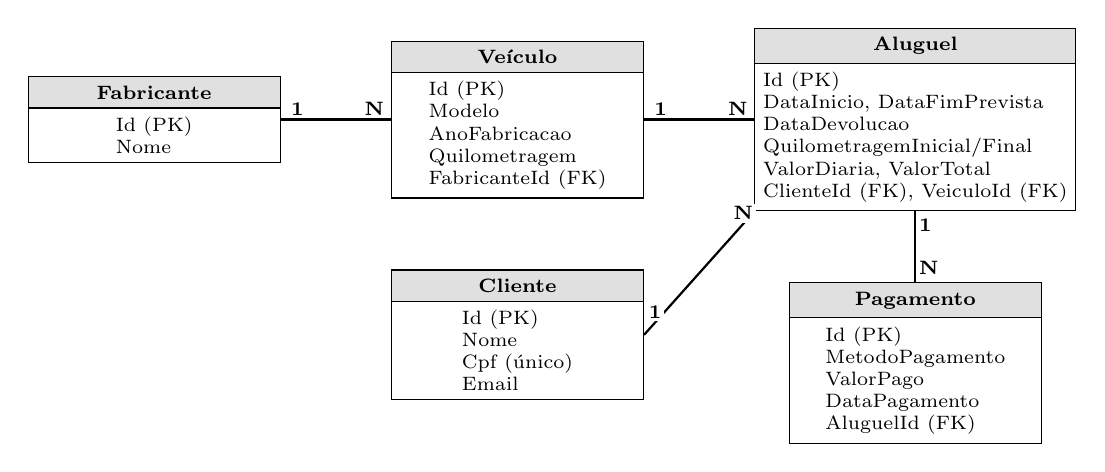
\begin{tikzpicture}[
  ent/.style={draw, rectangle split, rectangle split parts=2, rectangle split part fill={black!12,white},
              font=\scriptsize, align=left, inner sep=3pt, minimum width=3.2cm},
  rel/.style={-, thick},
  card/.style={font=\scriptsize\bfseries, fill=white, inner sep=1pt}]
\node[ent] (fab) {\textbf{Fabricante}\nodepart{second}Id (PK)\\Nome};
\node[ent, right=1.4cm of fab] (vei) {\textbf{Veículo}\nodepart{second}Id (PK)\\Modelo\\AnoFabricacao\\Quilometragem\\FabricanteId (FK)};
\node[ent, right=1.4cm of vei] (alu) {\textbf{Aluguel}\nodepart{second}Id (PK)\\DataInicio, DataFimPrevista\\DataDevolucao\\QuilometragemInicial/Final\\ValorDiaria, ValorTotal\\ClienteId (FK), VeiculoId (FK)};
\node[ent, below=0.9cm of alu] (pag) {\textbf{Pagamento}\nodepart{second}Id (PK)\\MetodoPagamento\\ValorPago\\DataPagamento\\AluguelId (FK)};
\node[ent, below=0.9cm of vei] (cli) {\textbf{Cliente}\nodepart{second}Id (PK)\\Nome\\Cpf (único)\\Email};
\draw[rel] (fab) -- node[card, pos=0.15, above] {1} node[card, pos=0.85, above] {N} (vei);
\draw[rel] (vei) -- node[card, pos=0.15, above] {1} node[card, pos=0.85, above] {N} (alu);
\draw[rel] (cli.east) -- node[card, pos=0.1, above] {1} node[card, pos=0.9, above] {N} (alu.south west);
\draw[rel] (alu) -- node[card, pos=0.2, right] {1} node[card, pos=0.8, right] {N} (pag);
\end{tikzpicture}
\caption{Modelo de dados do RentalSystem (Trabalho Prático 1).}
\label{fig:er}
\end{figure}

\begin{table}[htbp]
\centering
\caption{Entidades e restrições principais.}
\label{tab:entidades}
\small
\begin{tabularx}{\linewidth}{@{}lX@{}}
\toprule
\textbf{Entidade} & \textbf{Atributos e restrições} \\
\midrule
Fabricante & Nome obrigatório (até 100 caracteres). \\
Veículo & Modelo, ano e quilometragem obrigatórios; chave estrangeira para Fabricante. \\
Cliente & Nome, CPF (formato 000.000.000-00, índice único) e e-mail obrigatórios. \\
Aluguel & Datas de início e de devolução prevista, km inicial e diária obrigatórios; devolução, km final e total preenchidos na devolução; chaves para Cliente e Veículo. \\
Pagamento & Método, valor e data obrigatórios; chave estrangeira para Aluguel. \\
\bottomrule
\end{tabularx}
\end{table}

\section{Arquitetura e tecnologias}
\label{sec:arquitetura}

O sistema segue uma arquitetura cliente-servidor em três camadas (Figura~\ref{fig:arquitetura}).
O navegador carrega páginas estáticas que, por meio da Fetch API~\cite{mdn-fetch}, trocam JSON com
a API ASP.NET Core~\cite{ms-aspnet}. Os \emph{controllers} da API usam o Entity Framework
Core~\cite{ms-efcore} para consultar e gravar no SQL Server Express.

\begin{figure}[htbp]
\centering
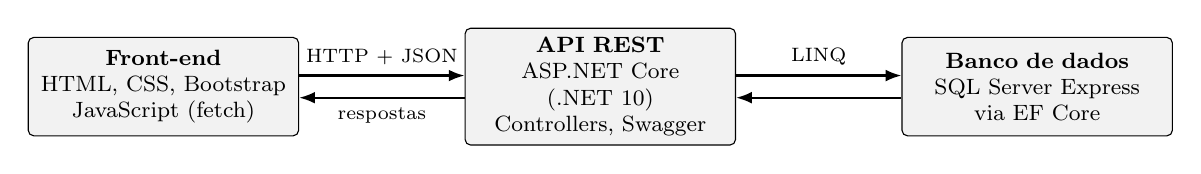
\begin{tikzpicture}[
  caixa/.style={draw, rounded corners=2pt, align=center, font=\footnotesize, minimum height=1.25cm, text width=3.2cm, fill=black!5},
  seta/.style={-{Latex[length=2mm]}, thick}]
\node[caixa] (front) {\textbf{Front-end}\\HTML, CSS, Bootstrap\\JavaScript (fetch)};
\node[caixa, right=2.1cm of front] (api) {\textbf{API REST}\\ASP.NET Core (.NET 10)\\Controllers, Swagger};
\node[caixa, right=2.1cm of api] (bd) {\textbf{Banco de dados}\\SQL Server Express\\via EF Core};
\draw[seta] ([yshift=4pt]front.east) -- node[above, font=\scriptsize] {HTTP + JSON} ([yshift=4pt]api.west);
\draw[seta] ([yshift=-4pt]api.west) -- node[below, font=\scriptsize] {respostas} ([yshift=-4pt]front.east);
\draw[seta] ([yshift=4pt]api.east) -- node[above, font=\scriptsize] {LINQ} ([yshift=4pt]bd.west);
\draw[seta] ([yshift=-4pt]bd.east -| bd.west) -- ([yshift=-4pt]api.east);
\end{tikzpicture}
\caption{Arquitetura do RentalSystem.}
\label{fig:arquitetura}
\end{figure}

Seguindo as regras do trabalho, o front-end usa apenas HTML, CSS, Bootstrap~5~\cite{bootstrap} e
JavaScript, sem etapa de compilação. Cada tela é um arquivo HTML com um script próprio, e o arquivo
\texttt{js/comum.js} reúne o que todas compartilham: o endereço da API, as funções de requisição
(\texttt{buscarJSON} e \texttt{enviarJSON}), a formatação de moeda, datas e quilometragem, os avisos
(\emph{toasts}), a validação de formulários e o modal de confirmação de exclusão.
O Código~\ref{cod:fetch} mostra a função usada em todas as pesquisas: os filtros preenchidos viram
parâmetros da URL e as respostas de erro da API são convertidas em mensagens legíveis.

\begin{lstlisting}[language=JS, caption={Função de pesquisa compartilhada (\texttt{comum.js}).}, label={cod:fetch}]
async function buscarJSON(caminho, filtros) {
  let params = new URLSearchParams();
  for (let [campo, valor] of Object.entries(filtros || {})) {
    if (valor !== undefined && valor !== null && String(valor).trim() !== "")
      params.set(campo, String(valor).trim());
  }
  let query = params.toString();
  let resposta = await fetch(urlBase + caminho + (query ? "?" + query : ""));
  if (!resposta.ok) throw await erroDaResposta(resposta);
  return resposta.json();
}
\end{lstlisting}

O front-end fica em uma pasta própria, \texttt{RentalSystem.Front}, ao lado do projeto da API
(\texttt{RentalSystem}), mantendo a estrutura do Trabalho Prático~1.

\section{Wireframes}
\label{sec:wireframes}

Antes da implementação, as telas foram desenhadas no Figma como wireframes de média fidelidade em
tons de cinza. Para manter o mesmo padrão em todas as telas, foram criados componentes reutilizáveis
(barra de navegação, botões, campos de formulário e etiquetas de status). A Tabela~\ref{tab:wireframes}
lista as dez telas e a Figura~\ref{fig:wireframe} mostra o wireframe da tela inicial.

\begin{table}[htbp]
\centering
\caption{Telas desenhadas nos wireframes.}
\label{tab:wireframes}
\small
\begin{tabularx}{\linewidth}{@{}lX@{}}
\toprule
\textbf{Tela} & \textbf{Conteúdo} \\
\midrule
01 Início & Indicadores, aluguéis em aberto e atalhos \\
02--06 Cadastros & Fabricantes, Veículos, Clientes, Aluguéis e Pagamentos: título, botão de novo registro, painel de filtros e tabela com ações \\
07 Consultas & Abas com as cinco consultas, SQL equivalente e tabela de resultado \\
08 Modal de veículo & Formulário de cadastro e edição \\
09 Modal de aluguel & Formulário com cálculo do valor estimado \\
10 Modal de devolução & Data, km final e valor total calculado \\
\bottomrule
\end{tabularx}
\end{table}

\begin{figure}[htbp]
\centering
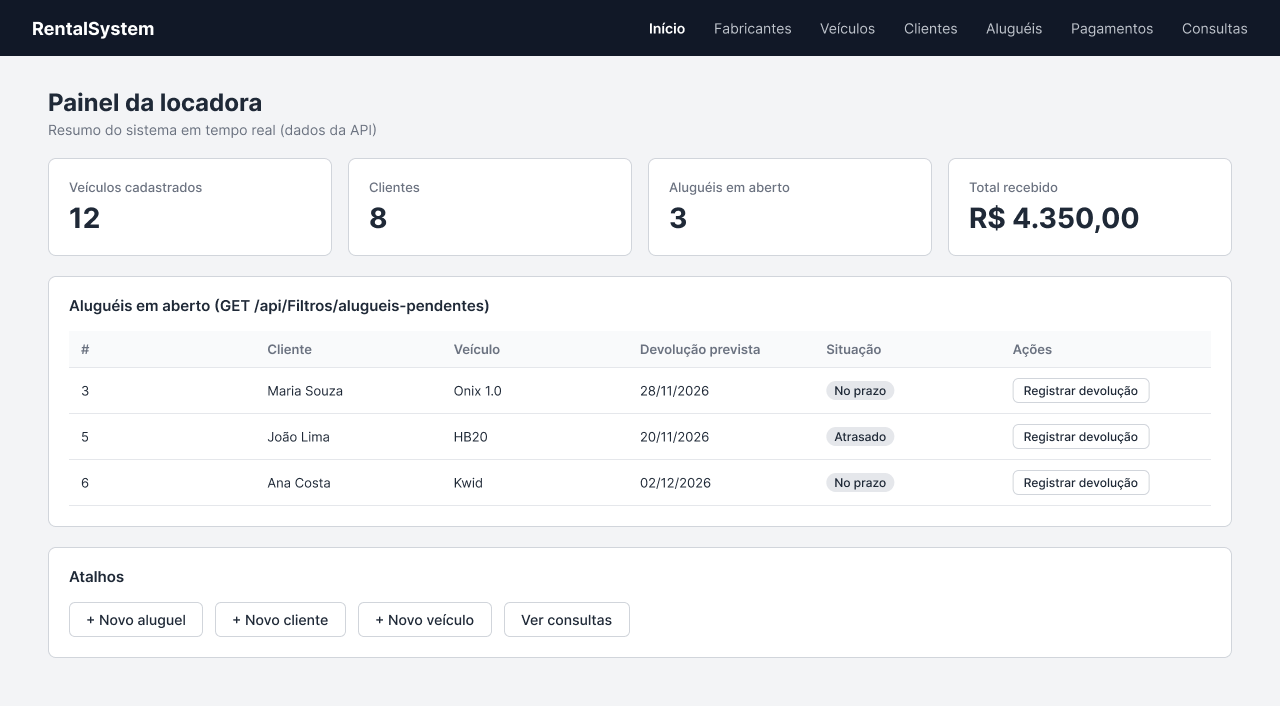
\includegraphics[width=0.92\linewidth]{wireframe-inicio.png}
\caption{Wireframe da tela inicial (Figma).}
\label{fig:wireframe}
\end{figure}

\section{Implementação do front-end}
\label{sec:implementacao}

\subsection{Telas e rotas utilizadas}

Todas as telas de cadastro seguem o mesmo padrão: um cabeçalho com o total de registros, um painel
de filtros, a tabela com os botões \emph{Editar} e \emph{Excluir} e um modal com o formulário.
A Tabela~\ref{tab:telas} relaciona cada tela às rotas da API que ela consome.

\begin{table}[htbp]
\centering
\caption{Telas do front-end e rotas da API consumidas.}
\label{tab:telas}
\small
\begin{tabularx}{\linewidth}{@{}l>{\raggedright\arraybackslash}X@{}}
\toprule
\textbf{Tela} & \textbf{Rotas} \\
\midrule
Início & \texttt{GET} Veiculos, Clientes, Alugueis, Pagamentos; \texttt{GET} Filtros/alugueis-pendentes \\
Fabricantes & \texttt{GET/POST/PUT/DELETE} Fabricantes; \texttt{GET} Veiculos (quantidade por fabricante) \\
Veículos & \texttt{GET/POST/PUT/DELETE} Veiculos; \texttt{GET} Fabricantes; \texttt{GET} Alugueis?status=aberto \\
Clientes & \texttt{GET/POST/PUT/DELETE} Clientes; \texttt{GET} Alugueis \\
Aluguéis & \texttt{GET/POST/PUT/DELETE} Alugueis; \texttt{GET} Clientes, Veiculos; \texttt{PUT} Veiculos (devolução) \\
Pagamentos & \texttt{GET/POST/PUT/DELETE} Pagamentos; \texttt{GET} Alugueis, Clientes, Veiculos \\
Consultas & \texttt{GET} das cinco rotas de \texttt{/api/Filtros} \\
\bottomrule
\end{tabularx}
\end{table}

\begin{figure}[htbp]
\centering
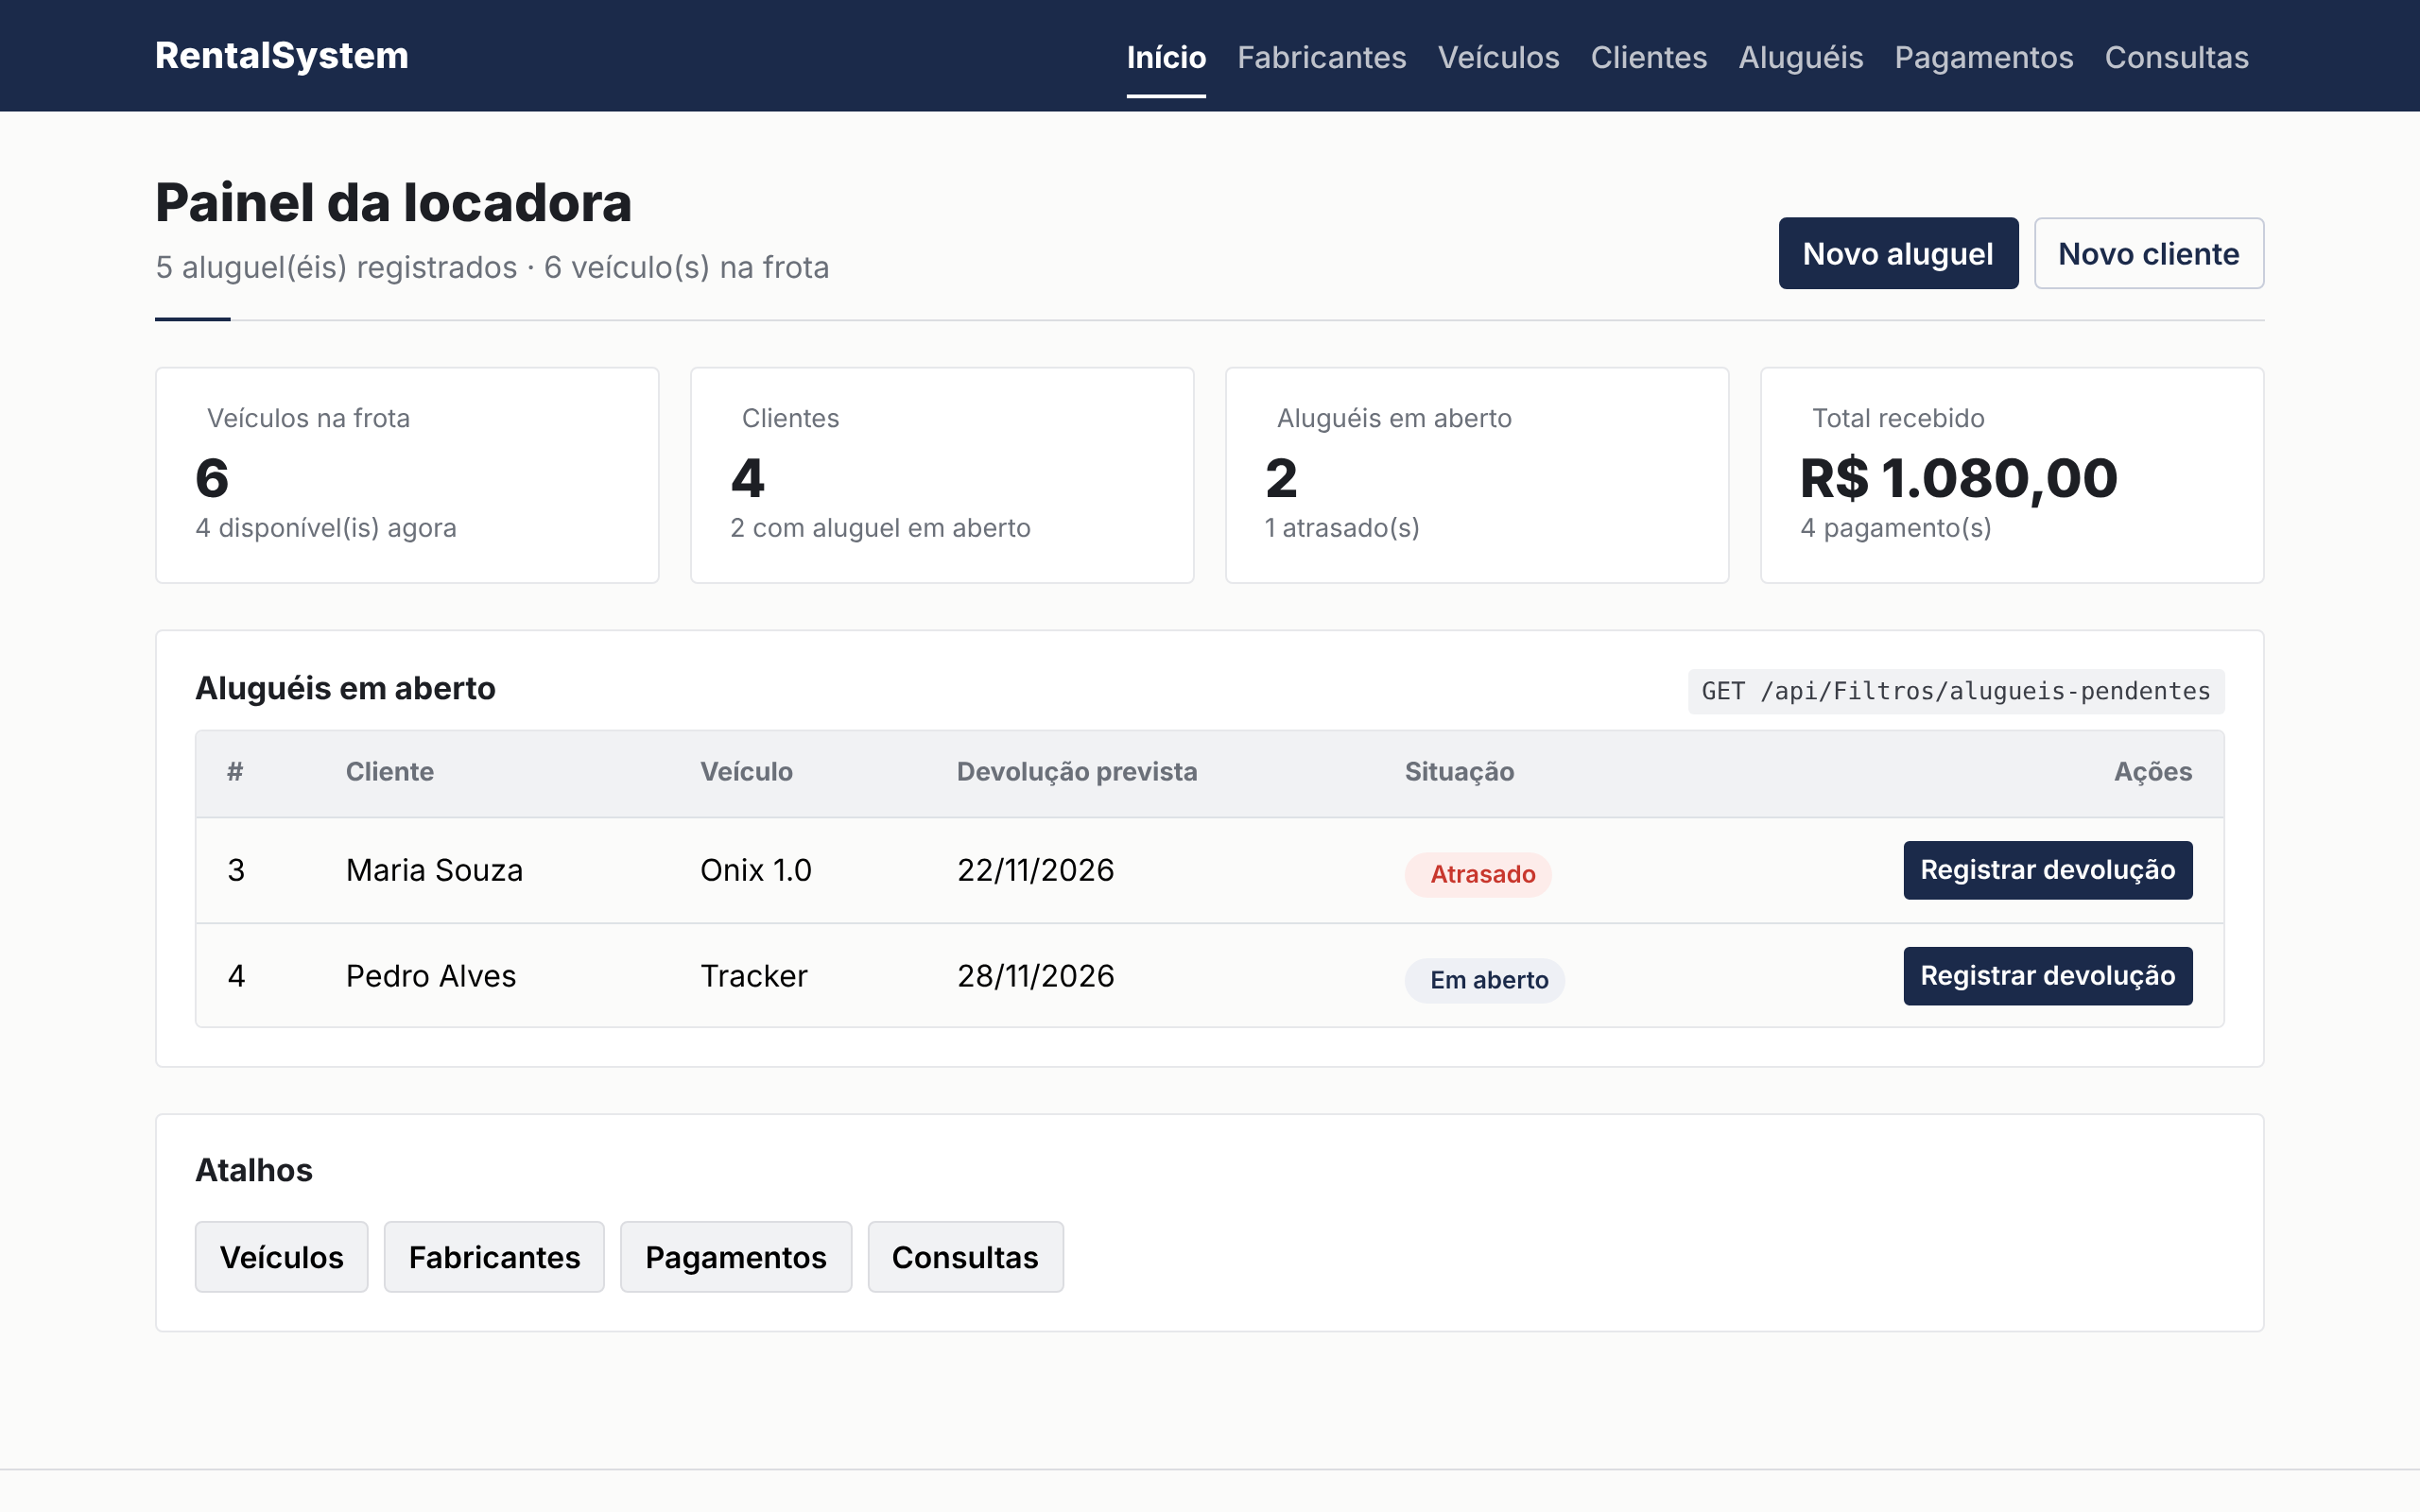
\includegraphics[width=0.92\linewidth]{front-inicio.png}
\caption{Tela inicial implementada (dados de exemplo).}
\label{fig:inicio}
\end{figure}

\subsection{Filtros personalizados}

Os métodos \texttt{GET} da API do Trabalho Prático~1 devolviam sempre a lista completa. Para que a
pesquisa acontecesse no banco, e não apenas no navegador, cada um recebeu parâmetros opcionais e
combináveis (Tabela~\ref{tab:filtros}). O Código~\ref{cod:filtro} mostra o caso dos veículos: cada
parâmetro informado acrescenta uma condição à consulta, que o Entity Framework traduz para uma
cláusula \texttt{WHERE}.

\begin{table}[htbp]
\centering
\caption{Filtros disponíveis por entidade.}
\label{tab:filtros}
\small
\begin{tabularx}{\linewidth}{@{}l>{\raggedright\arraybackslash}X@{}}
\toprule
\textbf{Entidade} & \textbf{Parâmetros de pesquisa} \\
\midrule
Fabricantes & \texttt{nome}, \texttt{comVeiculos} \\
Veículos & \texttt{modelo}, \texttt{fabricanteId}, \texttt{anoMin}, \texttt{anoMax}, \texttt{kmMax} \\
Clientes & \texttt{nome}, \texttt{cpf}, \texttt{email} \\
Aluguéis & \texttt{clienteId}, \texttt{veiculoId}, \texttt{status}, \texttt{dataInicioDe}, \texttt{dataInicioAte} \\
Pagamentos & \texttt{aluguelId}, \texttt{metodo}, \texttt{valorMin}, \texttt{dataDe}, \texttt{dataAte} \\
\bottomrule
\end{tabularx}
\end{table}

\begin{lstlisting}[language=CSharp, caption={Filtros do \texttt{GET /api/Veiculos} (trecho).}, label={cod:filtro}]
var query = _context.Veiculos.AsQueryable();
if (!string.IsNullOrWhiteSpace(modelo))
    query = query.Where(v => v.Modelo.Contains(modelo));
if (fabricanteId.HasValue)
    query = query.Where(v => v.FabricanteId == fabricanteId.Value);
if (anoMin.HasValue) query = query.Where(v => v.AnoFabricacao >= anoMin.Value);
if (anoMax.HasValue) query = query.Where(v => v.AnoFabricacao <= anoMax.Value);
if (kmMax.HasValue) query = query.Where(v => v.Quilometragem <= kmMax.Value);
var veiculos = await query.OrderBy(v => v.Modelo).ToListAsync();
\end{lstlisting}

\begin{figure}[htbp]
\centering
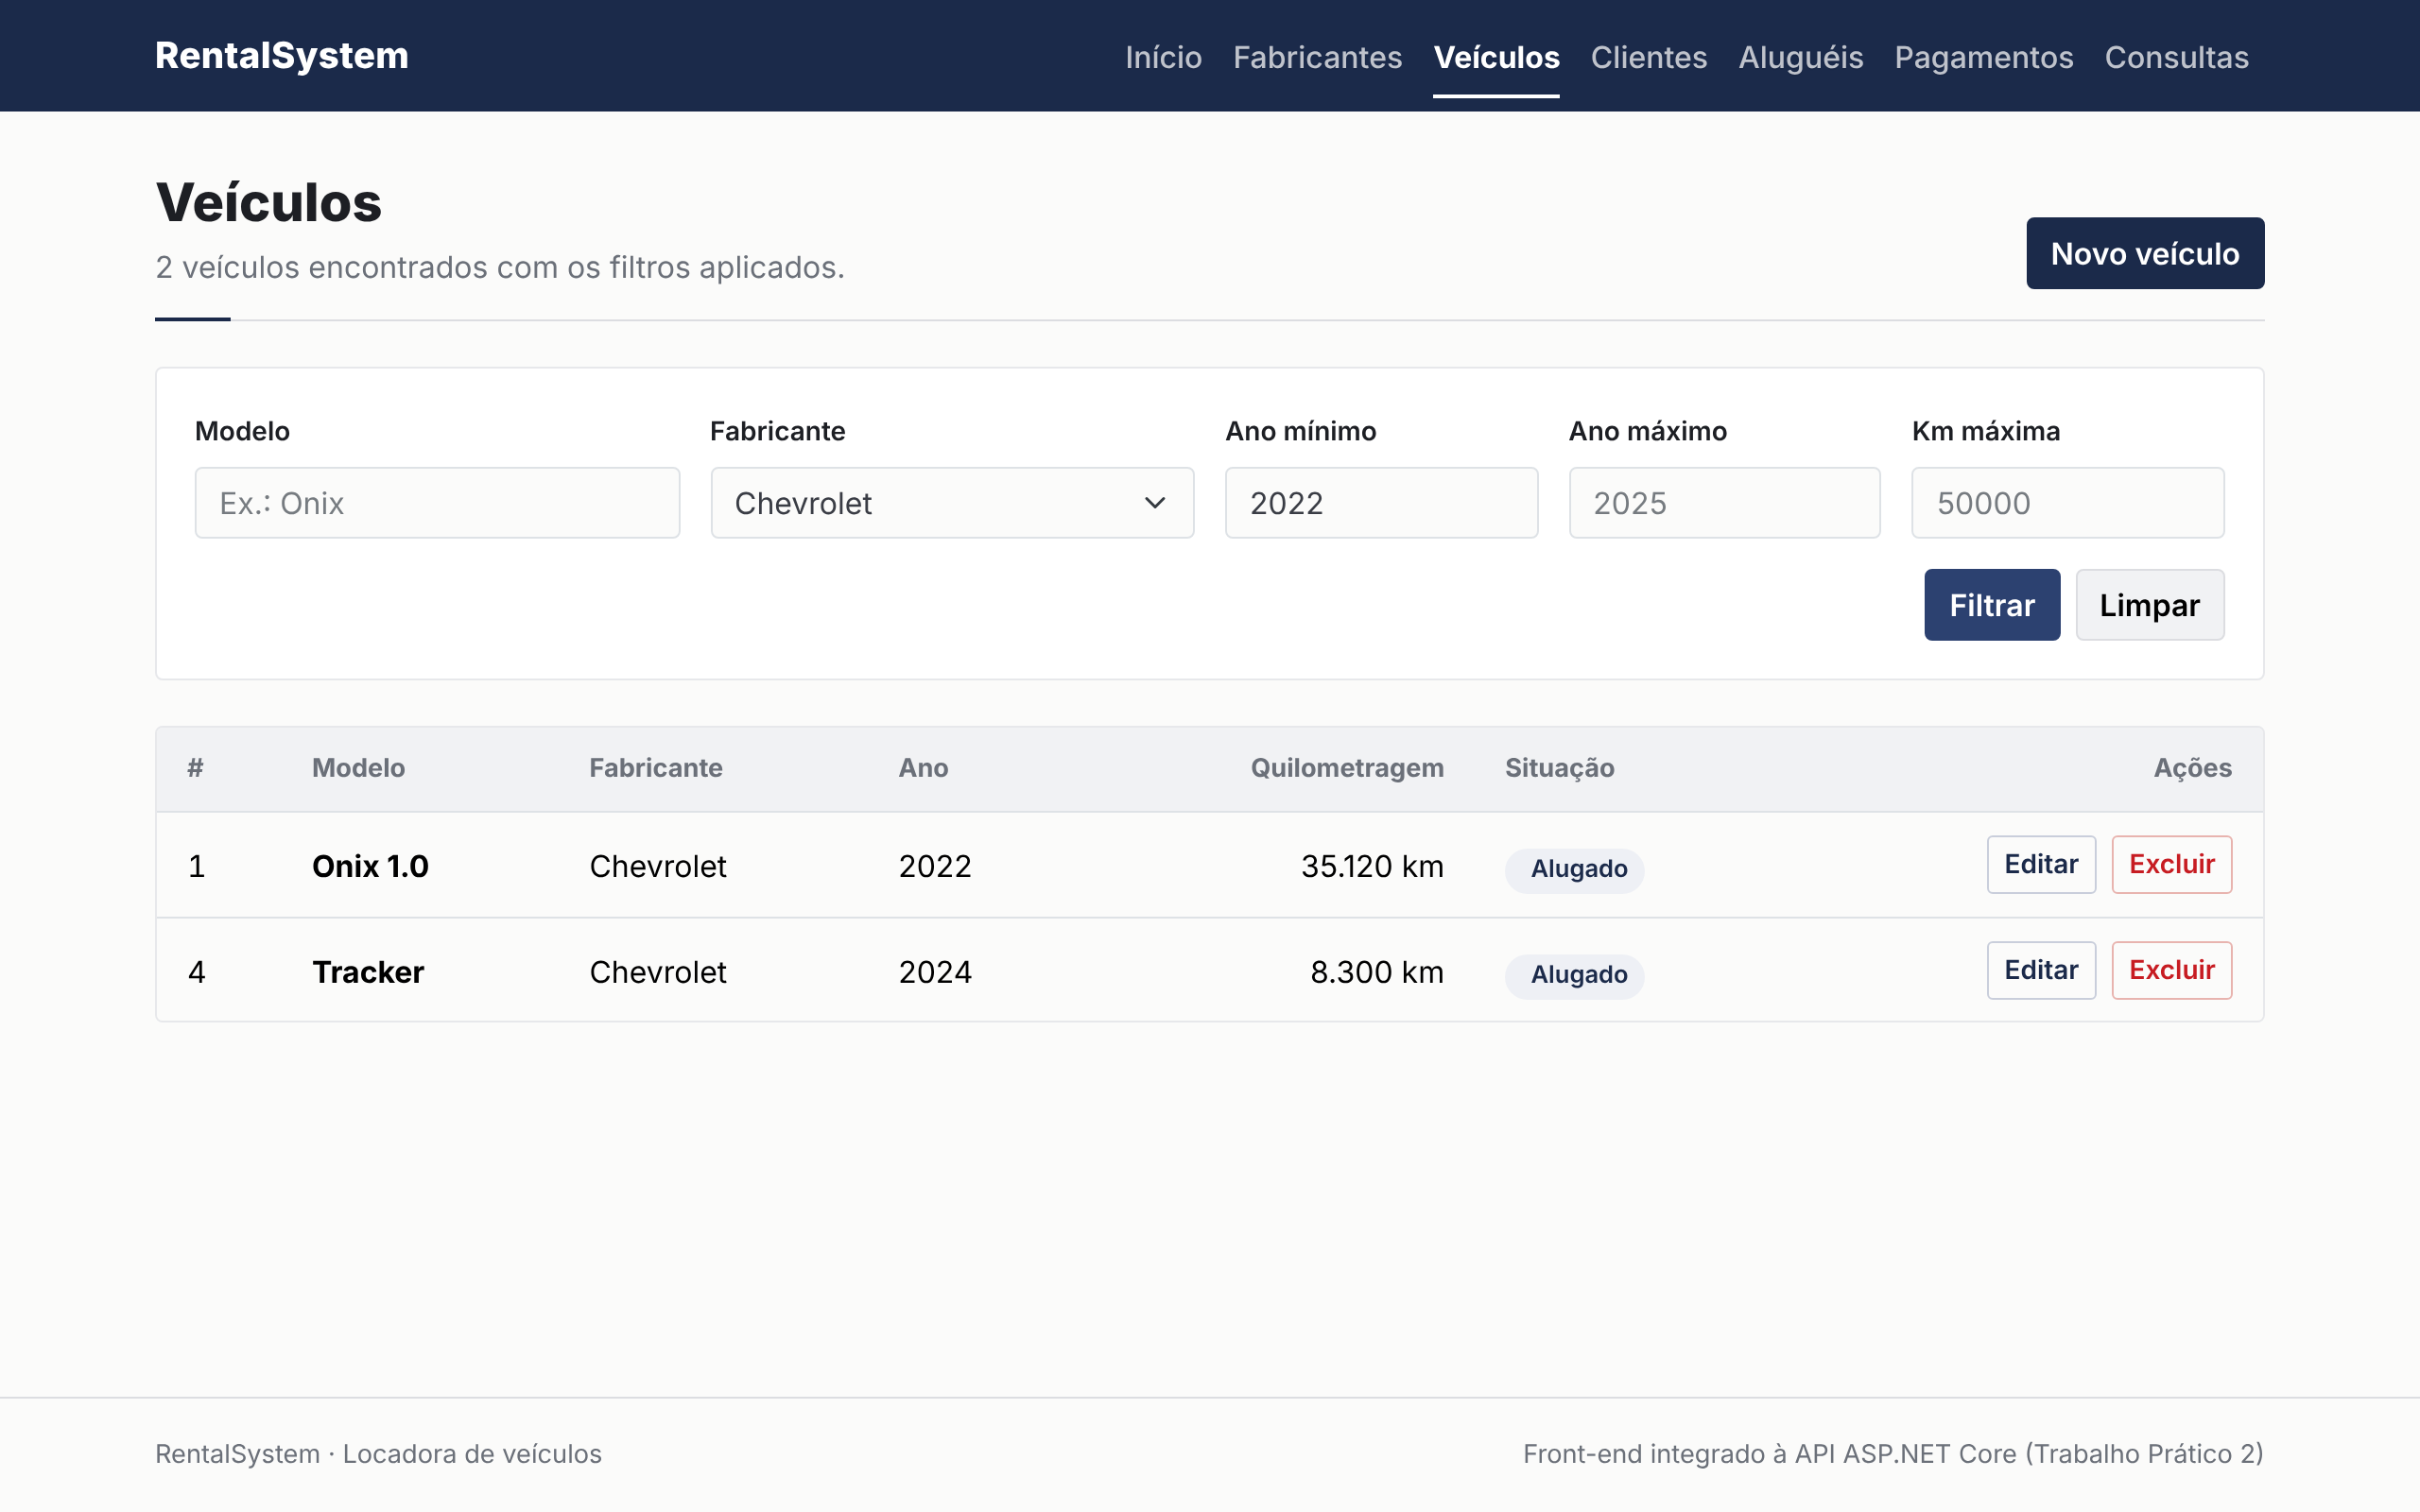
\includegraphics[width=0.92\linewidth]{front-veiculos-filtro.png}
\caption{Pesquisa de veículos filtrada por fabricante e ano mínimo (dados de exemplo).}
\label{fig:filtro}
\end{figure}

\subsection{Validações e tratamento de erros}

Antes de chamar a API, o front-end confere os campos obrigatórios e os limites de cada formulário.
Também aplica regras do negócio: CPF com máscara e dígitos verificadores válidos; devolução prevista
igual ou posterior ao início; km final não menor que a inicial; um veículo com aluguel em aberto não
pode ser alugado de novo; e o valor de um pagamento não pode passar do saldo do aluguel.
Os erros aparecem ao lado de cada campo (Figura~\ref{fig:validacao}). As respostas de erro da API
(400, 404, 409 e 500) são exibidas no próprio formulário ou em um aviso, e a falta de conexão
com a API gera uma mensagem específica.

\begin{figure}[htbp]
\centering
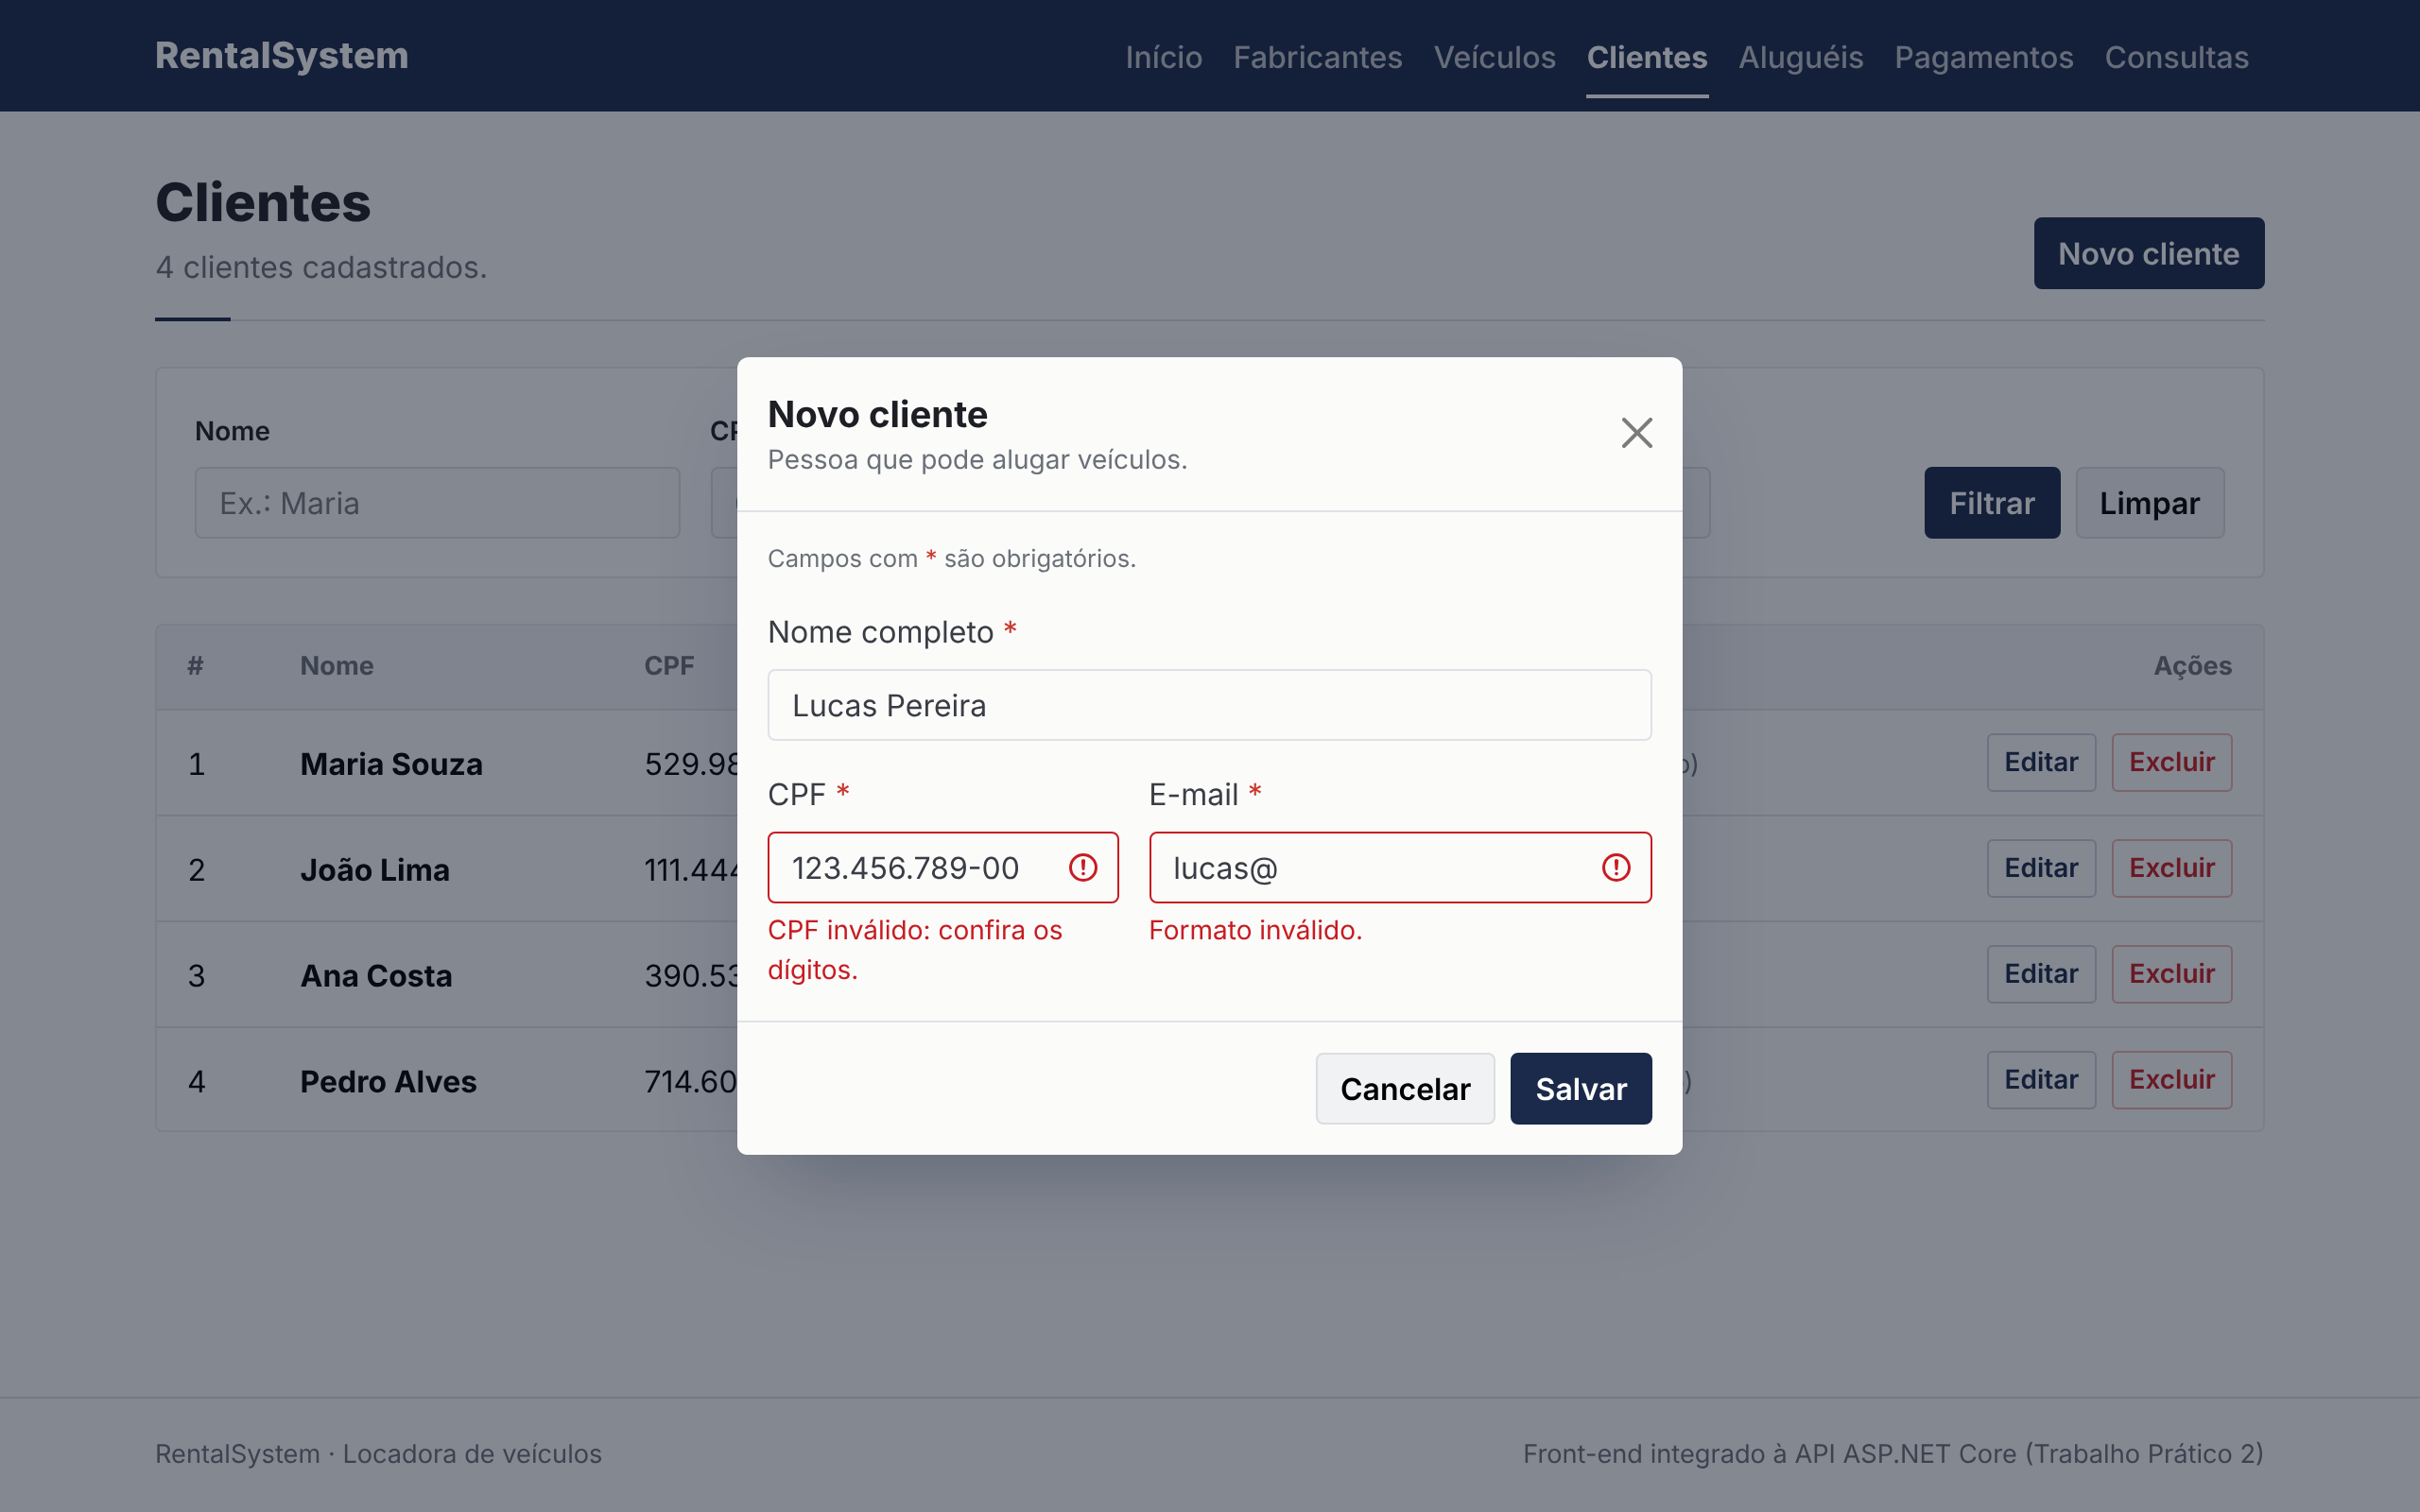
\includegraphics[width=0.88\linewidth]{front-validacao-cliente.png}
\caption{Validação do cadastro de cliente: CPF com dígitos inválidos e e-mail incompleto.}
\label{fig:validacao}
\end{figure}

\subsection{Registro de devolução}

A devolução é o principal fluxo da locadora. Ao clicar em \emph{Devolução}, o atendente informa a
data e a quilometragem final, e a tela mostra o valor total, calculado pela Equação~\ref{eq:diarias},
e a distância percorrida (Figura~\ref{fig:devolucao}). Ao confirmar, o front-end faz um
\texttt{PUT} no aluguel com a devolução, a km final e o valor total, e outro \texttt{PUT} no veículo
para atualizar a quilometragem dele.
\begin{equation}
\label{eq:diarias}
\textit{total} = \max\left(1, \left\lceil \textit{dataDevolucao} - \textit{dataInicio} \right\rceil_{\text{dias}}\right) \times \textit{valorDiaria}
\end{equation}

\begin{figure}[htbp]
\centering
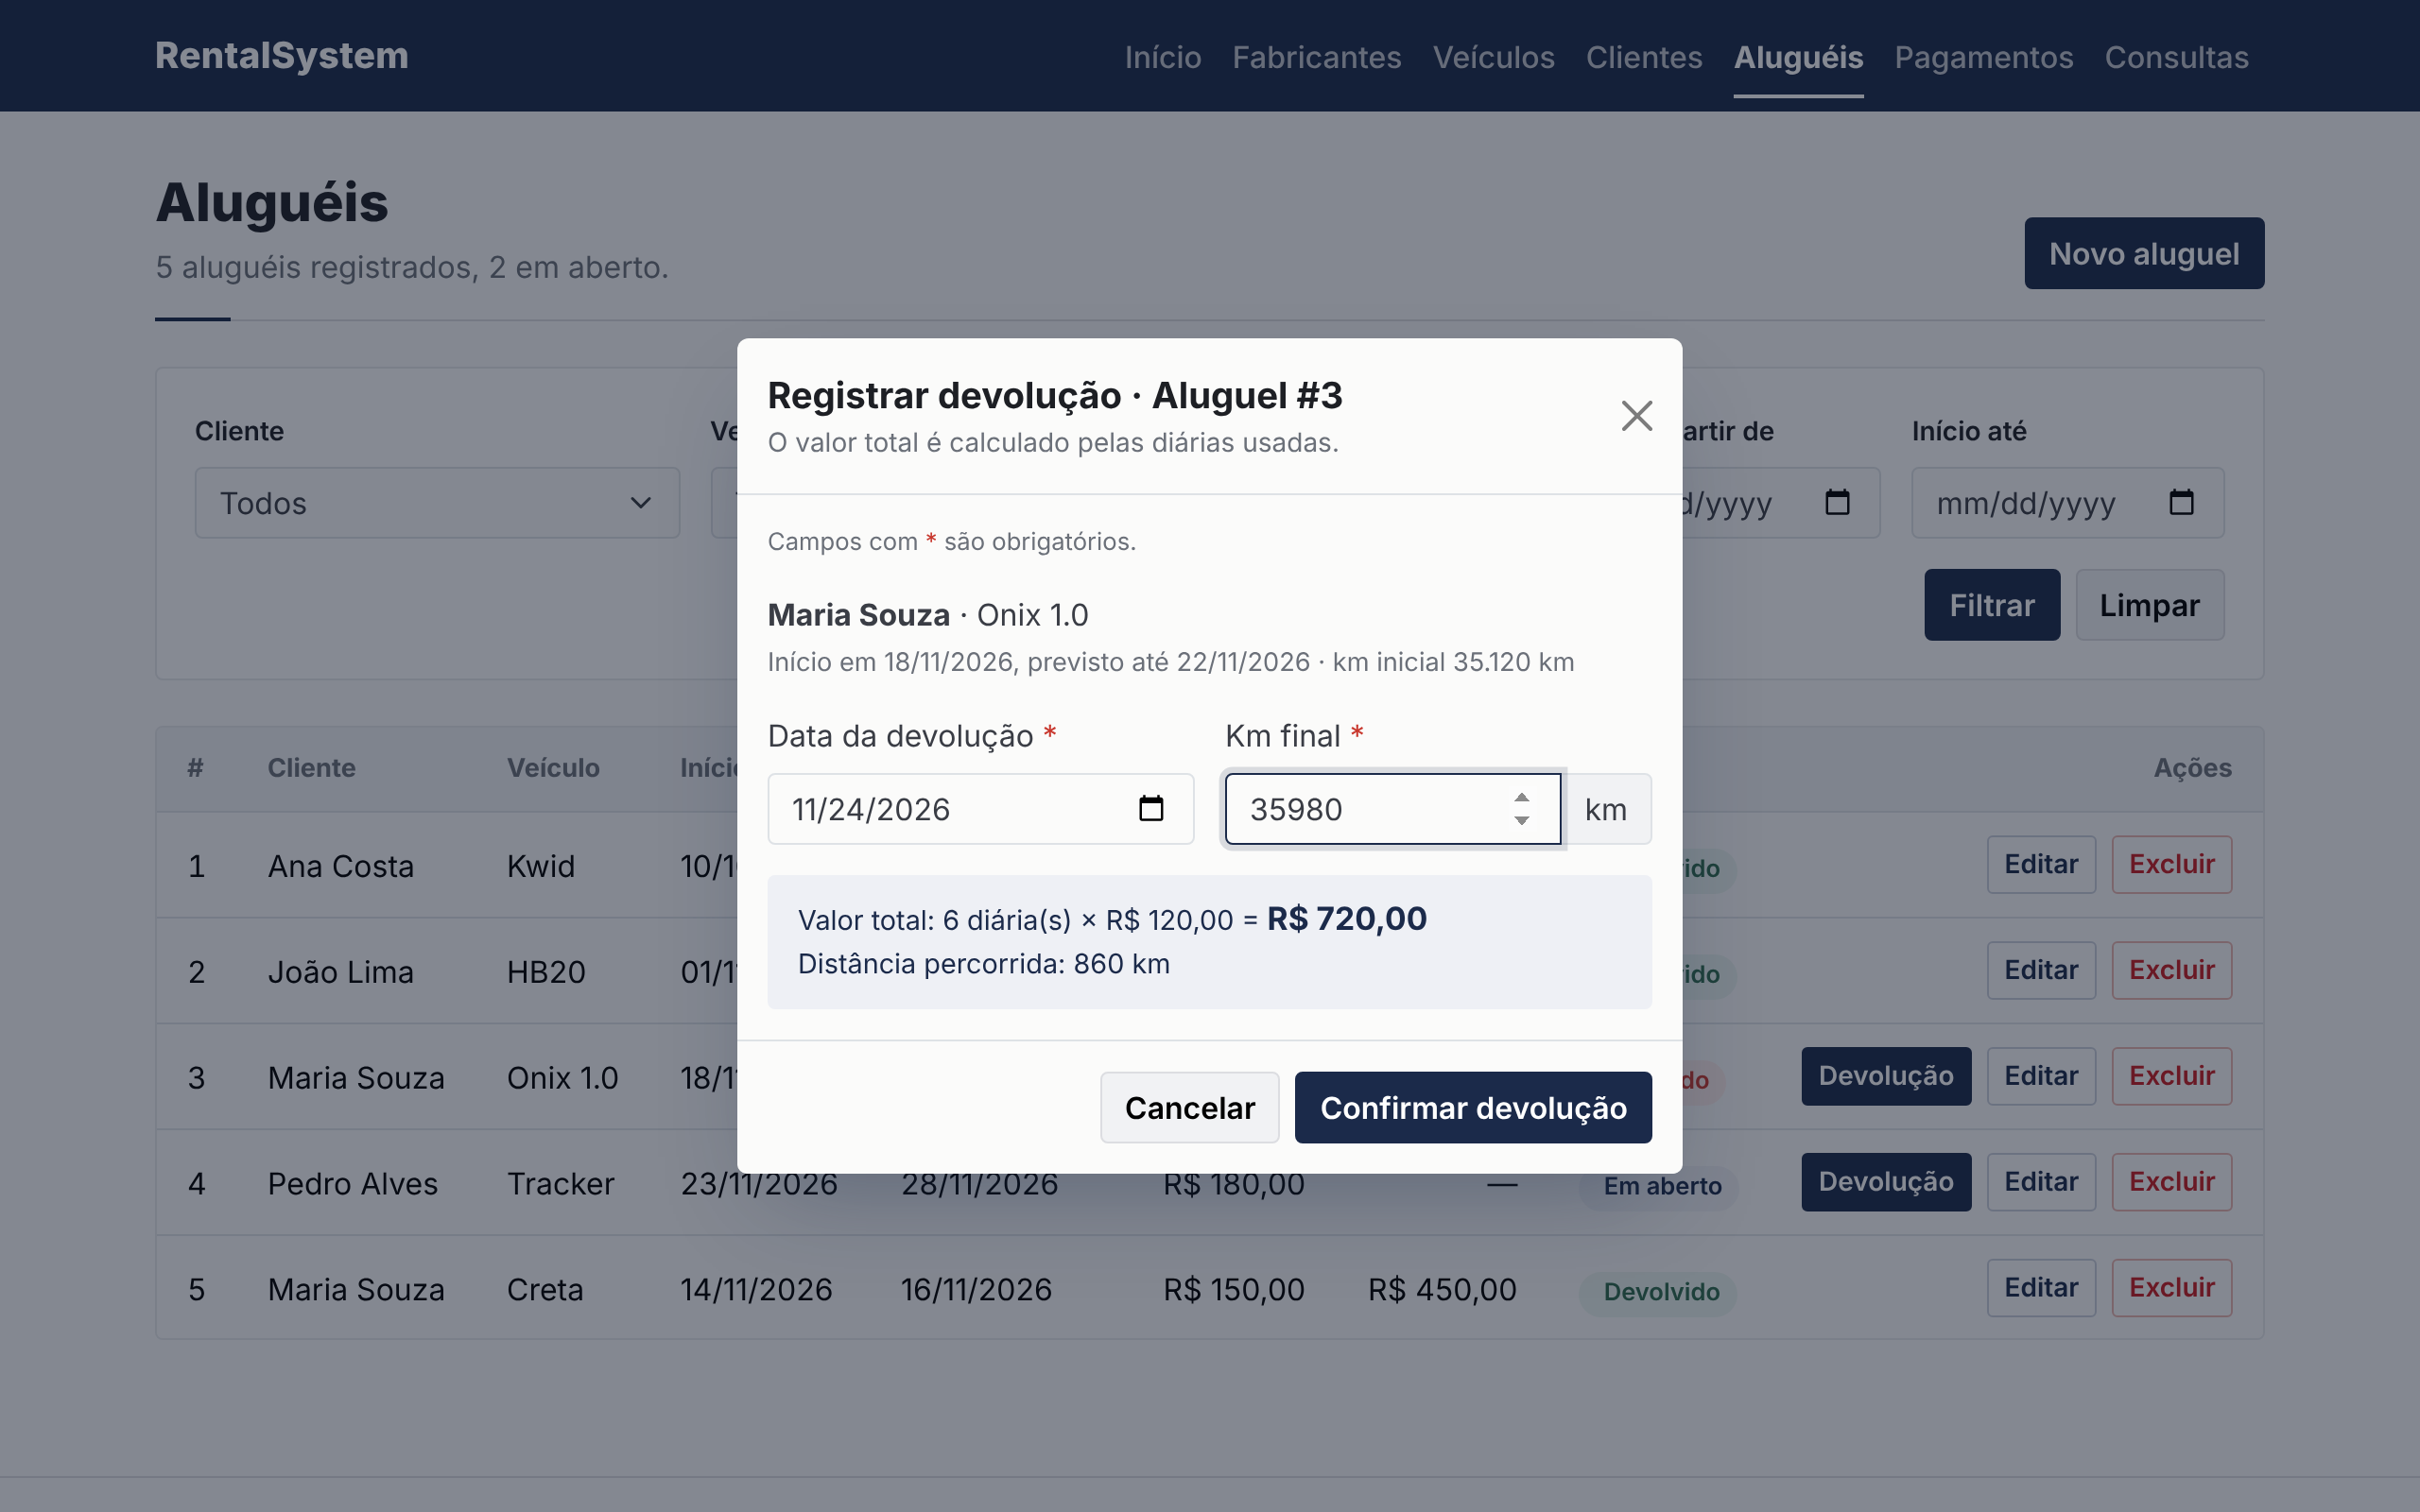
\includegraphics[width=0.88\linewidth]{front-devolucao.png}
\caption{Modal de registro de devolução com o cálculo do valor total.}
\label{fig:devolucao}
\end{figure}

\subsection{Ajustes no back-end}

Além dos filtros, dois ajustes foram necessários na API. O primeiro foi liberar o CORS no
\texttt{Program.cs}, porque o navegador bloqueia requisições de uma página para uma API em outra
origem sem essa permissão. O segundo foi proteger a exclusão: as chaves estrangeiras foram criadas
com exclusão em cascata, então excluir um fabricante apagaria também os veículos, aluguéis e
pagamentos ligados a ele. Agora a API responde \texttt{409 Conflict} ao tentar excluir um
fabricante com veículos, um veículo ou cliente com aluguéis ou um aluguel com pagamentos, e o
front-end mostra o motivo ao usuário.

\section{Exemplos de consultas: do banco à tela}
\label{sec:consultas}

A tela de Consultas reúne as cinco rotas de \texttt{/api/Filtros} criadas no Trabalho Prático~1
(Tabela~\ref{tab:rotas}). Para cada uma, mostra a rota chamada, o SQL equivalente, o resultado em
tabela, uma busca dentro do resultado e o total quando há valores. Dois exemplos são detalhados a
seguir.

\begin{table}[htbp]
\centering
\caption{Rotas de consulta com junção de tabelas.}
\label{tab:rotas}
\small
\begin{tabularx}{\linewidth}{@{}>{\ttfamily\raggedright\arraybackslash}p{7cm}X@{}}
\toprule
\normalfont\textbf{Rota} & \textbf{Junção} \\
\midrule
veiculos-com-fabricantes & Veículo \texttt{INNER JOIN} Fabricante \\
alugueis-detalhados & Aluguel \texttt{INNER JOIN} Cliente e Veículo \\
clientes-pagamentos-linq & Cliente \texttt{JOIN} Aluguel \texttt{JOIN} Pagamento \\
alugueis-pendentes & Aluguel com Cliente e Veículo, sem devolução \\
fabricantes-veiculos-leftjoin & Fabricante \texttt{LEFT JOIN} Veículo \\
\bottomrule
\end{tabularx}
\end{table}

\subsection{Aluguéis detalhados (INNER JOIN)}

A rota \texttt{GET /api/Filtros/alugueis-detalhados} junta cada aluguel ao cliente e ao veículo
correspondentes (Código~\ref{cod:inner}). No banco, isso equivale a dois \texttt{INNER JOIN}
(Código~\ref{cod:inner-sql}). No front-end, o resultado aparece com o total dos valores
(Figura~\ref{fig:inner}).

\begin{lstlisting}[language=CSharp, caption={Consulta \texttt{alugueis-detalhados} no controller.}, label={cod:inner}]
var alugueis = await _context.Alugueis
    .Include(a => a.Cliente)
    .Include(a => a.Veiculo)
    .Select(a => new {
        IdAluguel = a.Id, DataInicio = a.DataInicio,
        ClienteNome = a.Cliente!.Nome, VeiculoModelo = a.Veiculo!.Modelo,
        ValorTotal = a.ValorTotal
    }).ToListAsync();
\end{lstlisting}

\begin{lstlisting}[language=SQLsimples, caption={SQL equivalente.}, label={cod:inner-sql}]
SELECT a.Id, a.DataInicio, c.Nome AS ClienteNome,
       v.Modelo AS VeiculoModelo, a.ValorTotal
FROM Alugueis a
INNER JOIN Clientes c ON c.Id = a.ClienteId
INNER JOIN Veiculos v ON v.Id = a.VeiculoId
\end{lstlisting}

\begin{figure}[htbp]
\centering
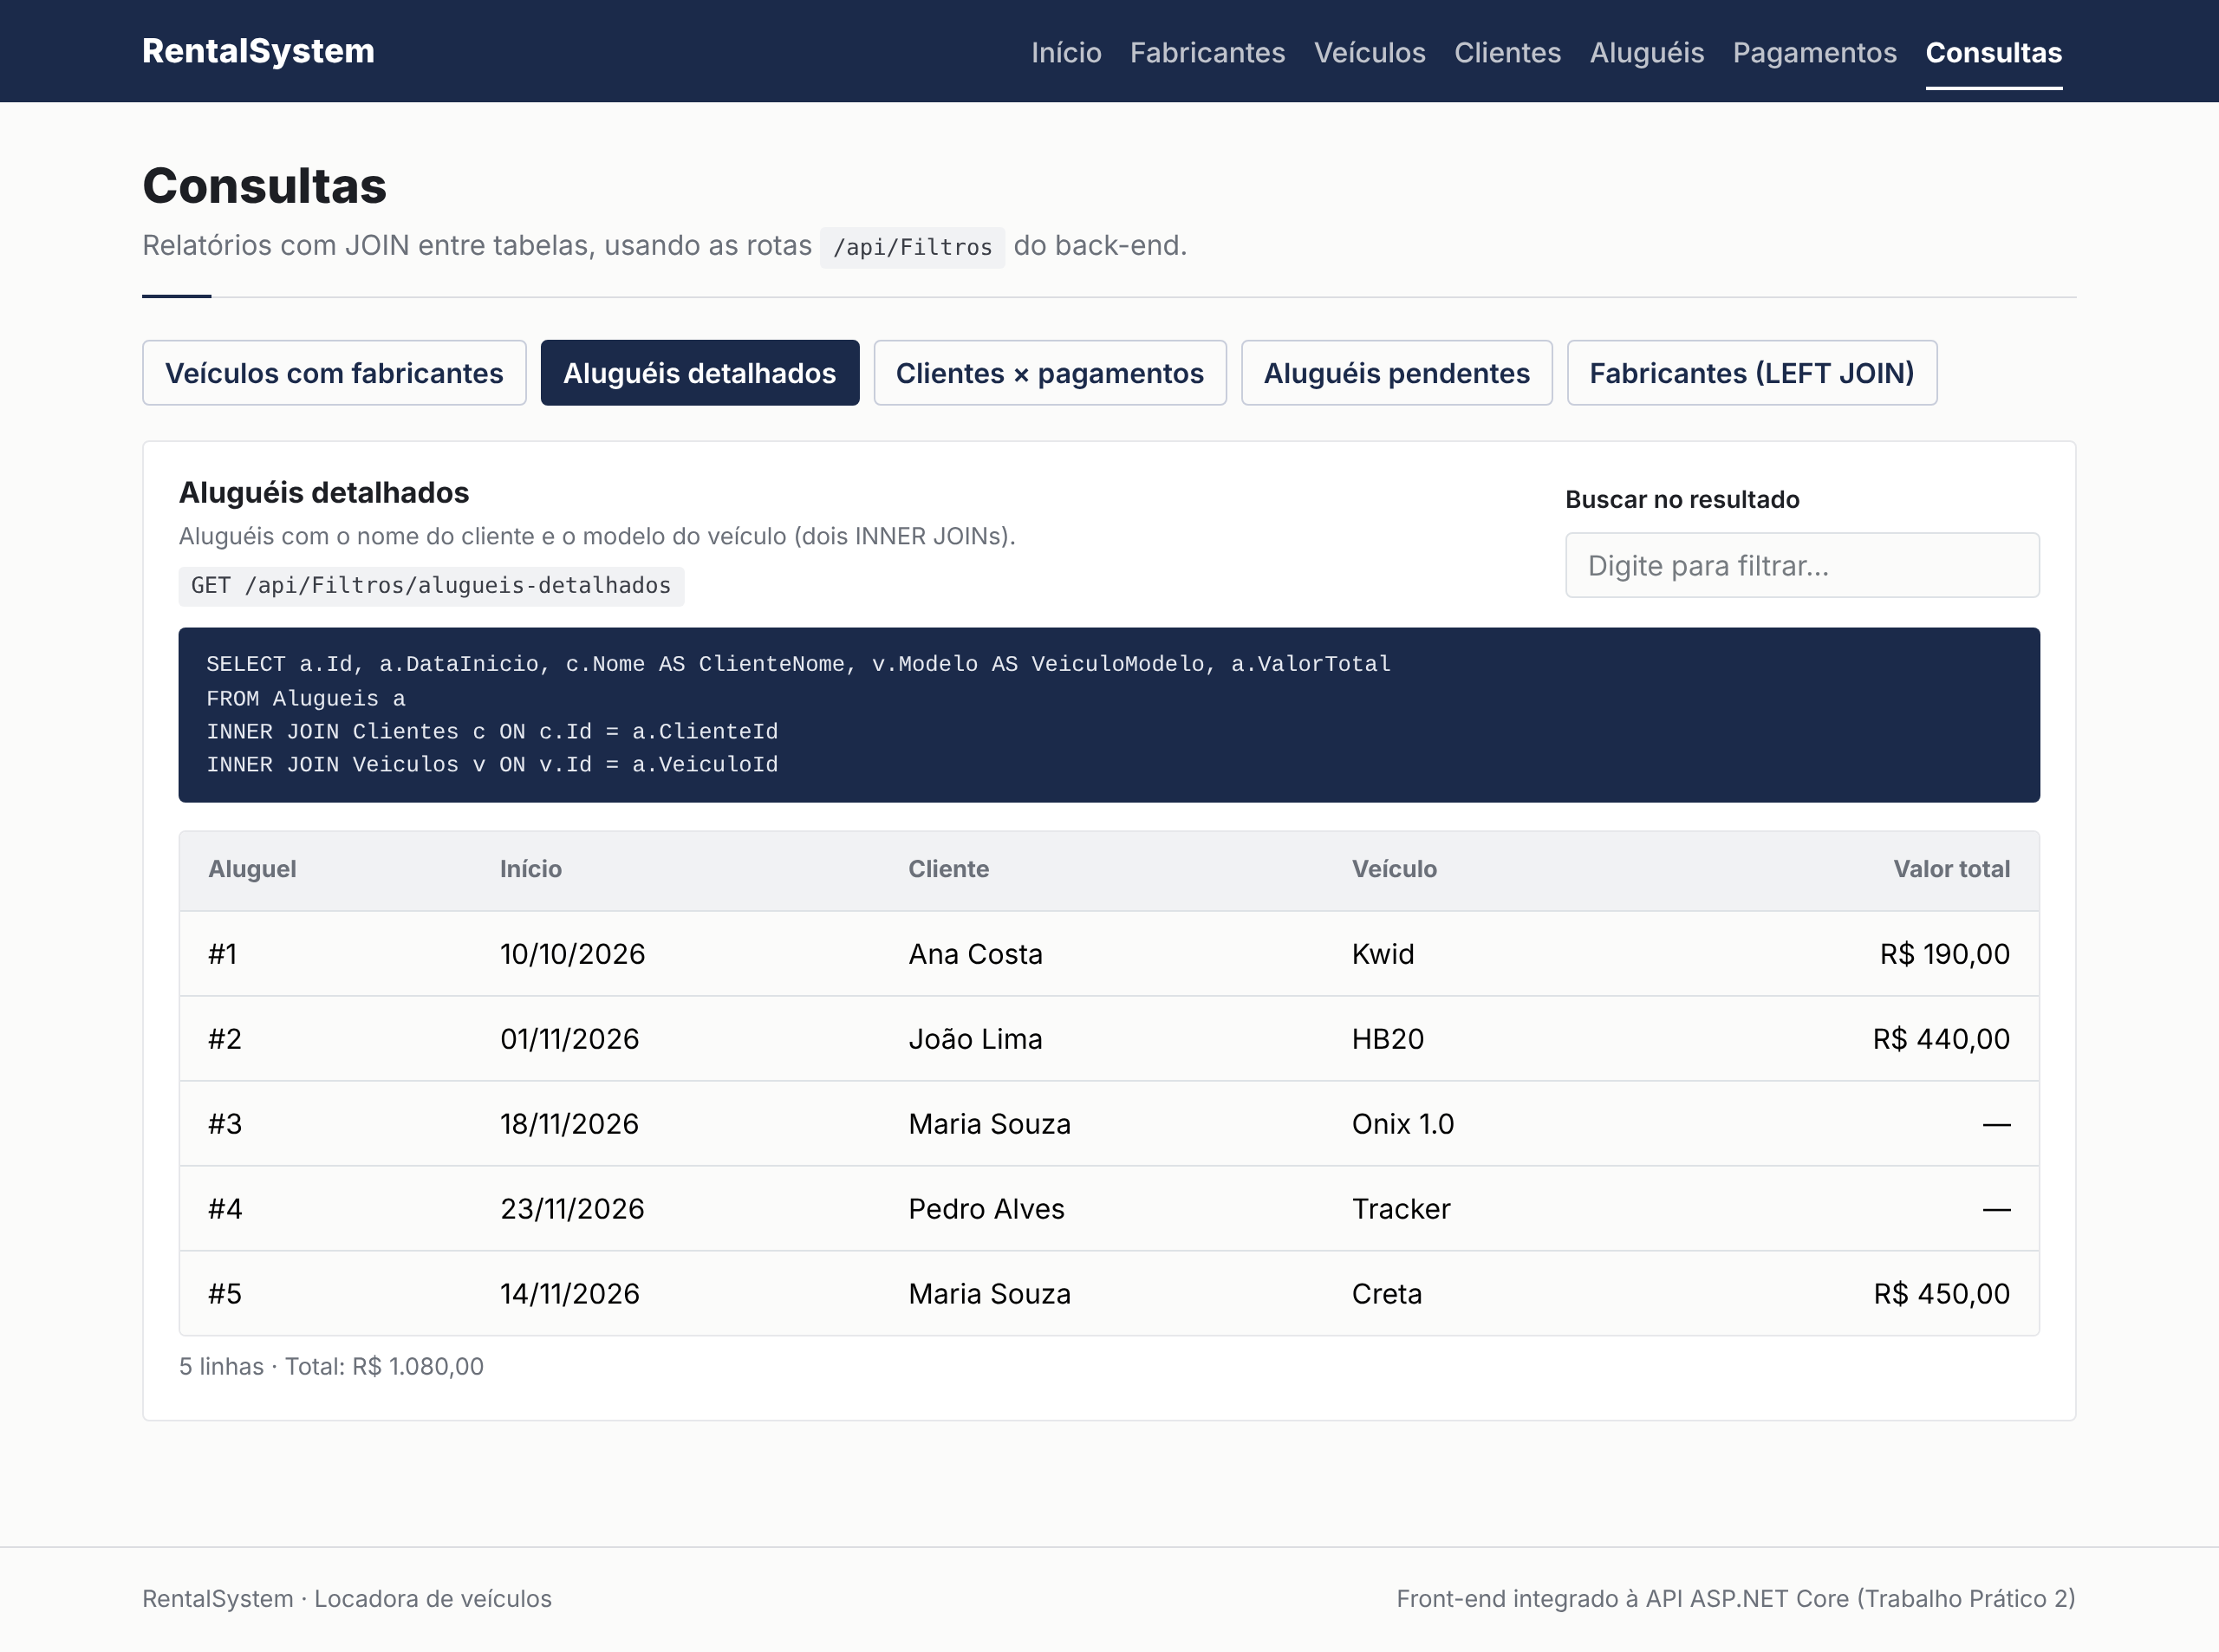
\includegraphics[width=0.88\linewidth]{front-consulta-detalhados.png}
\caption{Resultado da consulta de aluguéis detalhados no front-end.}
\label{fig:inner}
\end{figure}

\subsection{Fabricantes e veículos (LEFT JOIN)}

A rota \texttt{GET /api/Filtros/fabricantes-veiculos-leftjoin} lista todos os fabricantes, mesmo os
que ainda não têm veículos. Em LINQ, isso é feito com \texttt{join}/\texttt{into} seguido de
\texttt{DefaultIfEmpty()} (Código~\ref{cod:left}), o que equivale a um \texttt{LEFT JOIN}
\cite{elmasri}. Na tela, o fabricante sem veículos aparece com o texto ``Sem veículos''
(Figura~\ref{fig:left}).

\begin{lstlisting}[language=CSharp, caption={Consulta com LEFT JOIN em LINQ.}, label={cod:left}]
var query = await (
    from f in _context.Fabricantes
    join v in _context.Veiculos on f.Id equals v.FabricanteId into g
    from veiculo in g.DefaultIfEmpty()
    select new {
        Fabricante = f.Nome,
        Veiculo = veiculo == null ? "Sem veículos" : veiculo.Modelo
    }).ToListAsync();
\end{lstlisting}

\begin{figure}[htbp]
\centering
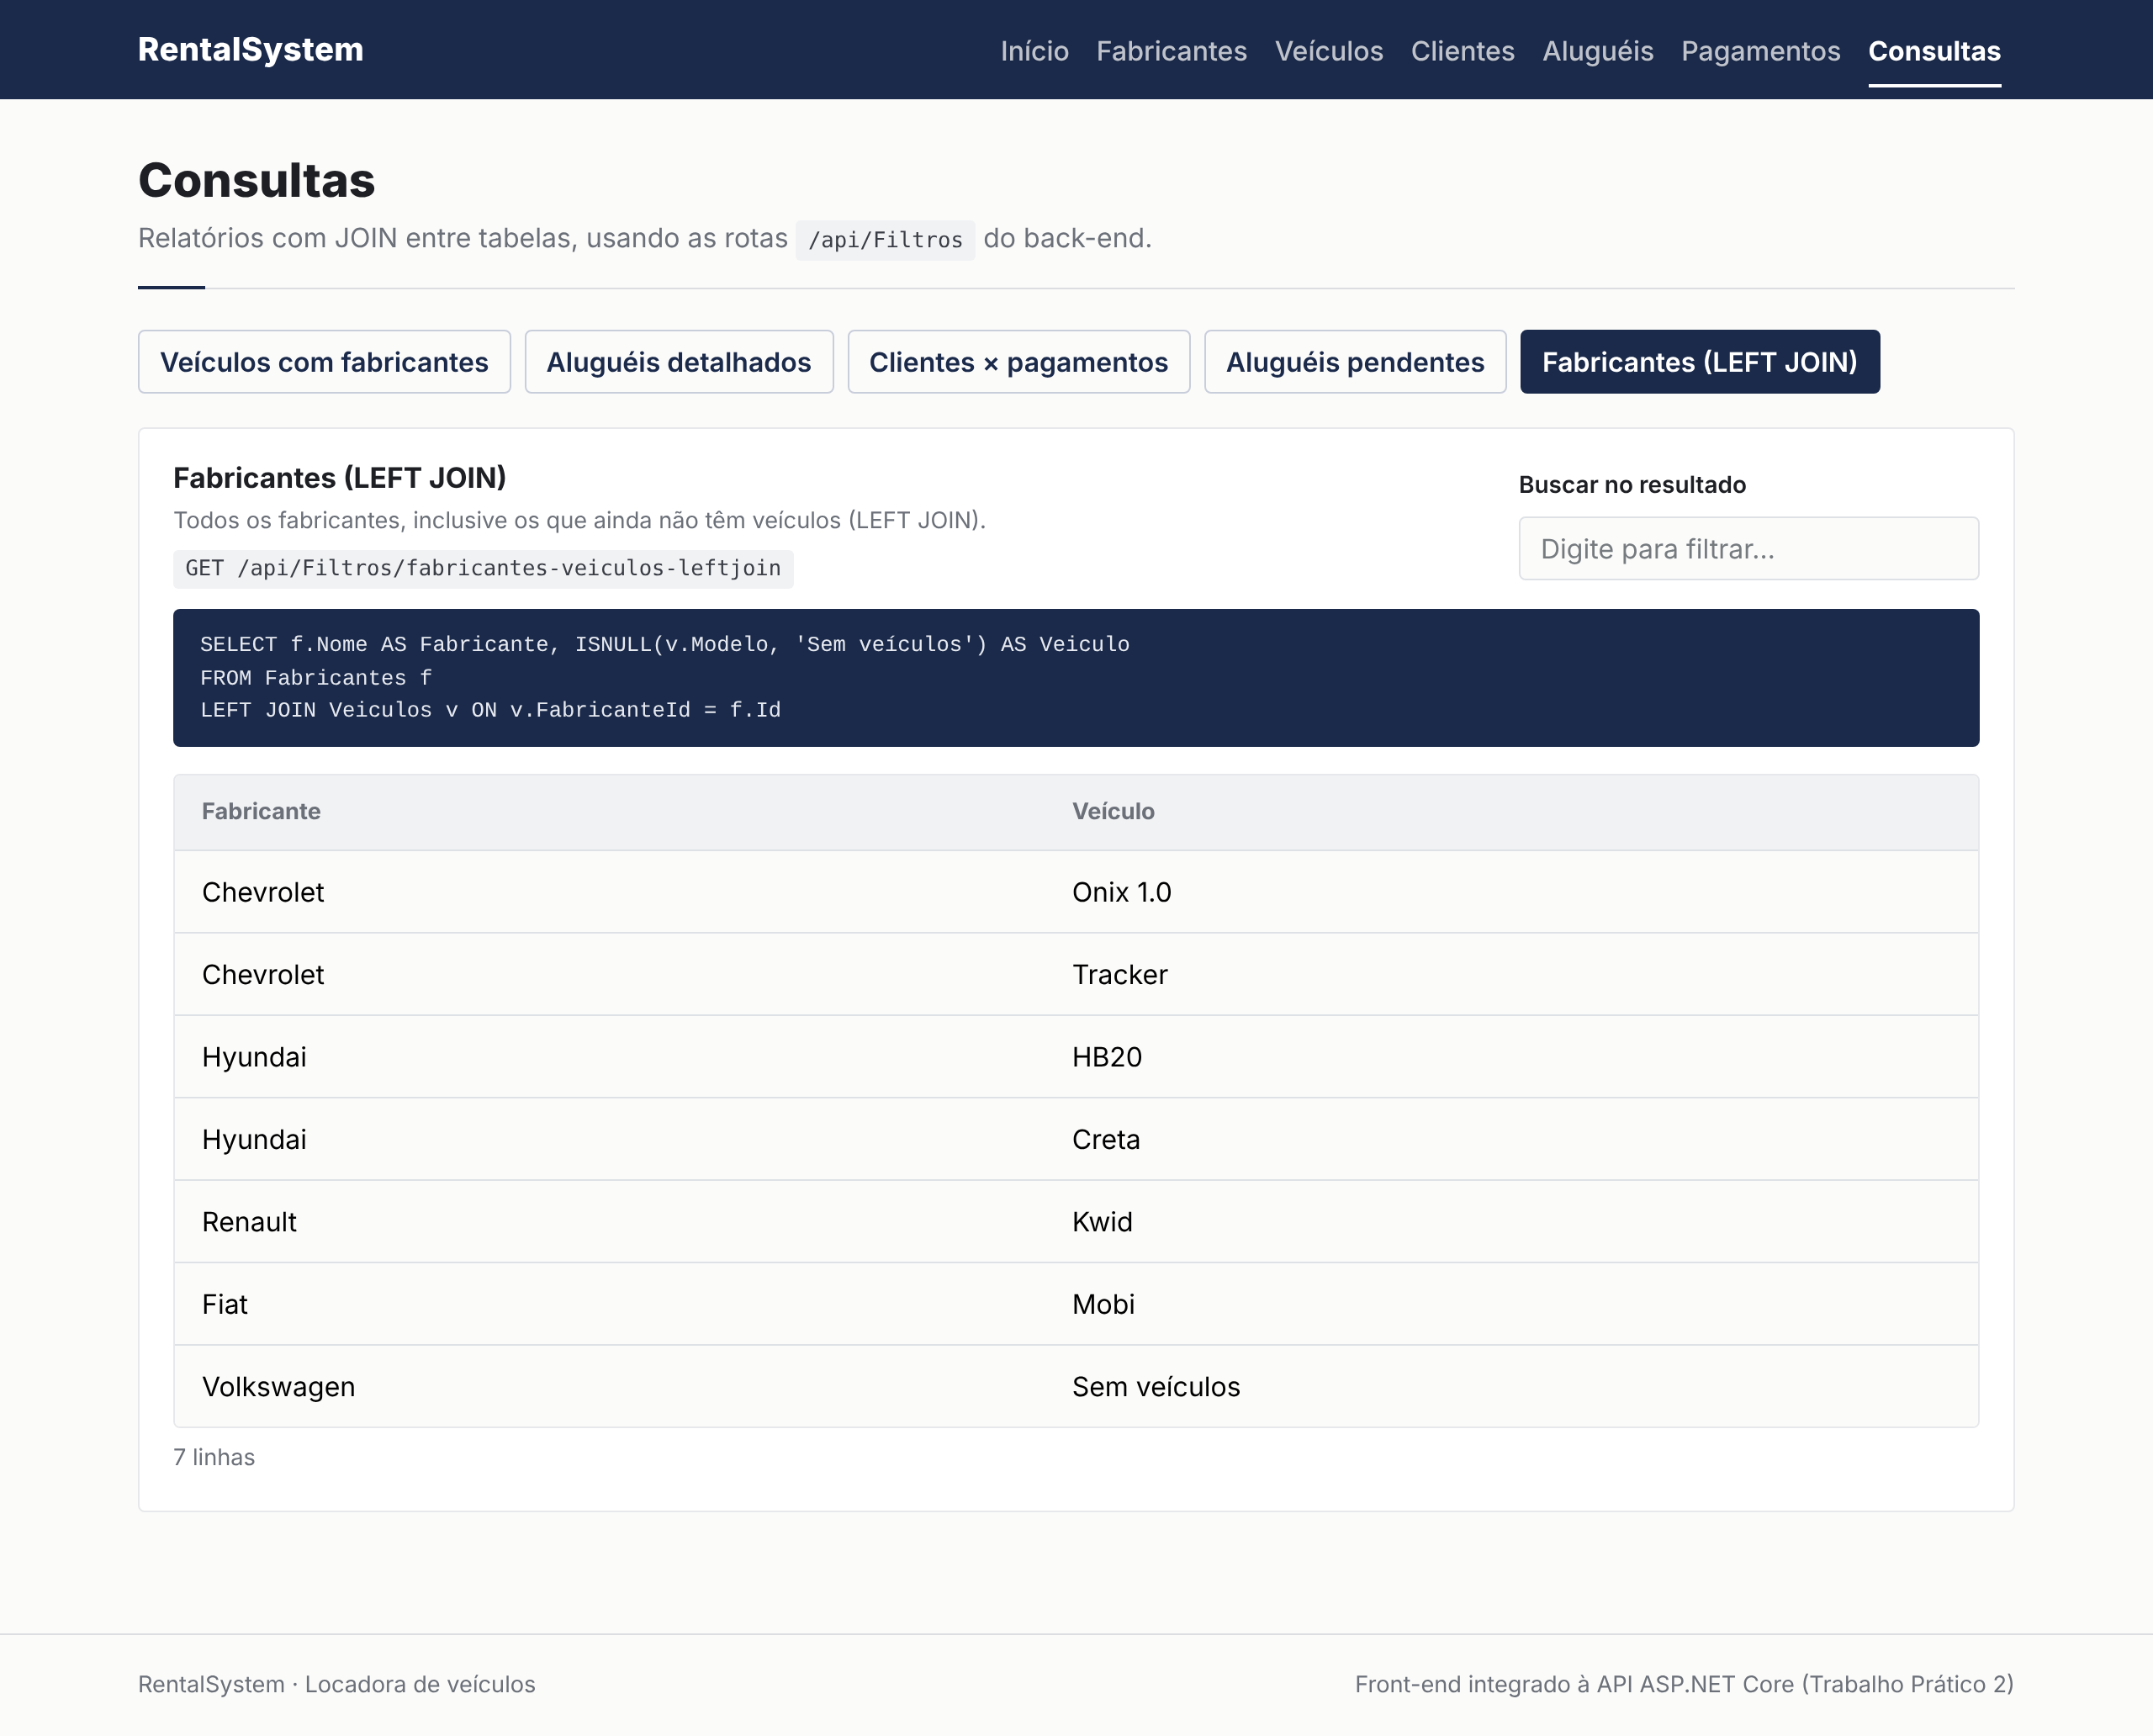
\includegraphics[width=0.88\linewidth]{front-consulta-leftjoin.png}
\caption{Resultado da consulta com LEFT JOIN: a Volkswagen ainda não tem veículos.}
\label{fig:left}
\end{figure}

\section{Testes}
\label{sec:testes}

As telas foram testadas manualmente no navegador, com a API em execução. A
Tabela~\ref{tab:testes} resume o roteiro de testes e o resultado esperado de cada cenário.

\begin{table}[htbp]
\centering
\caption{Roteiro de testes manuais.}
\label{tab:testes}
\small
\begin{tabularx}{\linewidth}{@{}>{\raggedright\arraybackslash}X>{\raggedright\arraybackslash}X@{}}
\toprule
\textbf{Cenário} & \textbf{Resultado esperado} \\
\midrule
Cadastrar, editar e excluir um registro em cada tela & Lista atualizada e aviso de sucesso \\
Salvar formulário com campos vazios & Campos marcados como obrigatórios, nada enviado à API \\
Combinar dois ou mais filtros e depois limpar & Lista filtrada pela API; ao limpar, lista completa \\
Cadastrar cliente com CPF inválido ou repetido & Erro no campo CPF (validação local ou 409 da API) \\
Excluir fabricante que possui veículos & Exclusão recusada com a mensagem da API (409) \\
Alugar veículo que já está alugado & Erro no campo Veículo \\
Registrar devolução com km menor que a inicial & Erro no campo Km final \\
Registrar devolução válida & Valor total calculado; km do veículo atualizada \\
Pagamento acima do saldo do aluguel & Erro no campo Valor pago \\
Abrir as cinco consultas & Resultados das rotas de \texttt{/api/Filtros} \\
Usar o sistema com a API desligada & Mensagem de falha de conexão em cada tela \\
\bottomrule
\end{tabularx}
\end{table}

\section{Considerações finais}
\label{sec:conclusao}

O trabalho entregou um front-end que cobre todas as funcionalidades do Trabalho Prático~1:
cadastro, edição, exclusão e pesquisa das cinco entidades, filtros em dois ou mais campos por
entidade executados no banco e as cinco consultas com junção exibidas em tela. A divisão entre o
\texttt{comum.js} e um script por tela manteve o código pequeno e fácil de explicar, sem
\emph{frameworks} além do Bootstrap. A integração também revelou problemas do back-end que passaram
despercebidos nos testes pelo Swagger, como a exclusão em cascata e a falta de CORS, que foram
corrigidos.

Como limitações, o sistema não tem autenticação, o cálculo do valor total da devolução é feito no
front-end e o Bootstrap é carregado por CDN, exigindo internet. Como trabalhos futuros, sugerem-se
login de atendentes, cálculo do total e atualização da quilometragem em uma única rota do
back-end (em transação), paginação das listas e reservas com data futura.

\begin{thebibliography}{99}

\bibitem[Bootstrap 2024]{bootstrap}
Bootstrap (2024). \emph{Bootstrap 5.3 documentation}. Disponível em:
\url{https://getbootstrap.com/docs/5.3/}. Acesso em: 24 nov. 2026.

\bibitem[Elmasri e Navathe 2018]{elmasri}
Elmasri, R. e Navathe, S. B. (2018). \emph{Sistemas de Banco de Dados}. 7. ed. São Paulo: Pearson.

\bibitem[MDN 2026]{mdn-fetch}
MDN Web Docs (2026). \emph{Fetch API}. Disponível em:
\url{https://developer.mozilla.org/pt-BR/docs/Web/API/Fetch_API}. Acesso em: 24 nov. 2026.

\bibitem[Microsoft 2026a]{ms-aspnet}
Microsoft (2026a). \emph{ASP.NET Core documentation}. Disponível em:
\url{https://learn.microsoft.com/aspnet/core/}. Acesso em: 24 nov. 2026.

\bibitem[Microsoft 2026b]{ms-efcore}
Microsoft (2026b). \emph{Entity Framework Core documentation}. Disponível em:
\url{https://learn.microsoft.com/ef/core/}. Acesso em: 24 nov. 2026.

\end{thebibliography}

\end{document}
